% Figure 2 — Conceptual workflow diagram
\documentclass[tikz,border=8pt]{standalone}
\usepackage{tikz}
\usetikzlibrary{shapes.geometric, arrows, positioning, fit, backgrounds, calc}

\begin{document}
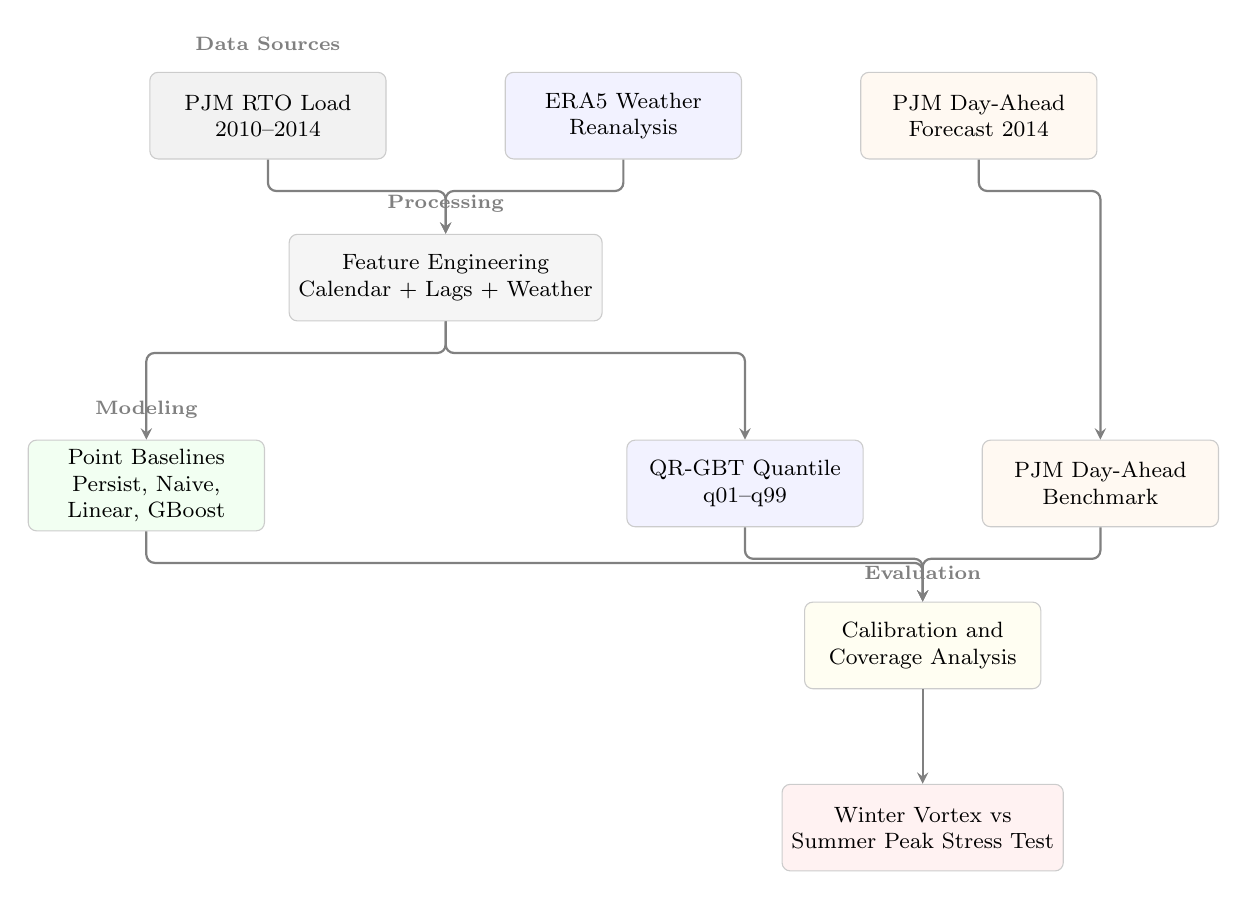
\begin{tikzpicture}[
    node distance=1.2cm and 1.0cm,
    box/.style={rectangle, rounded corners=3pt, draw=gray!40, fill=#1,
                minimum width=3.0cm, minimum height=1.1cm, align=center, font=\footnotesize},
    arrow/.style={->, >=stealth, gray, thick, rounded corners=3pt},
]

% ── Row 1: Data ──
\node[box=black!5] (pjm) {PJM RTO Load\\2010--2014};
\node[box=blue!5, right=1.5cm of pjm] (era5) {ERA5 Weather\\Reanalysis};
\node[box=orange!5, right=1.5cm of era5] (da) {PJM Day-Ahead\\Forecast 2014};

% ── Row 2: Feature Engineering ──
\node[box=gray!8, below=1.5cm of $(pjm)!0.5!(era5)$] (feat) {Feature Engineering\\Calendar + Lags + Weather};

% ── Row 3: Models ──
\node[box=green!5, below left=1.5cm and 0.3cm of feat] (point) {Point Baselines\\Persist, Naive,\\Linear, GBoost};
\node[box=blue!5, below right=1.5cm and 0.3cm of feat] (qr) {QR-GBT Quantile\\q01--q99};
\node[box=orange!5, right=1.5cm of qr] (bench) {PJM Day-Ahead\\Benchmark};

% ── Row 4: Evaluation ──
\node[box=yellow!5, below=1.5cm of $(qr)!0.5!(bench)$] (eval) {Calibration and\\Coverage Analysis};
\node[box=red!5, below=1.2cm of eval] (stress) {Winter Vortex vs\\Summer Peak Stress Test};

% ── Arrows ──
\draw[arrow] (pjm.south) -- ++(0,-0.4) -| (feat.north);
\draw[arrow] (era5.south) -- ++(0,-0.4) -| (feat.north);
\draw[arrow] (da.south) -- ++(0,-0.4) -| (bench.north);
\draw[arrow] (feat.south) -- ++(0,-0.4) -| (point.north);
\draw[arrow] (feat.south) -- ++(0,-0.4) -| (qr.north);
\draw[arrow] (point.south) -- ++(0,-0.4) -| (eval.north);
\draw[arrow] (qr.south) -- ++(0,-0.4) -| (eval.north);
\draw[arrow] (bench.south) -- ++(0,-0.4) -| (eval.north);
\draw[arrow] (eval.south) -- (stress.north);

% ── Labels ──
\node[font=\scriptsize\bfseries, gray, above=0.15cm of pjm] {Data Sources};
\node[font=\scriptsize\bfseries, gray, above=0.15cm of feat] {Processing};
\node[font=\scriptsize\bfseries, gray, above=0.15cm of point] {Modeling};
\node[font=\scriptsize\bfseries, gray, above=0.15cm of eval] {Evaluation};

\end{tikzpicture}
\end{document}
